\section{Desarollo packet pincer}

En esta sección veremos el funcionamiento de cada parte de la herramienta, la cual se ha llamado 'packet pincer' por el momento. Veremos qué y cuáles argumentos de consola acepta, como realiza la lectura de paquetes tanto en tiempo real como por trazas. A continuación se explicarán los diferentes pasos que llevan a cabo en el momento al analizar un paquete y como se realiza la generación de estadísticas. Finalmente, veremos como se realiza el etiquetado automático de los flujos y se escriben emiten los resultados.

El flujo principal de la aplicación se puede observar en la Figura \ref{fig:packet_pincer_execution}. Como podemos ver, se van extrayendo paquetes mientras se encuentren disponibles. Cuando se obtiene uno, en caso de ser un paquete IPv4 fragmentado, se intenta reconstruir o se guarda en caso de no poder. A continuación, se comprueba si la herramienta soporta analizar el paquete indicado y, en caso afirmativo, acumula la información en el flujo de transporte respectivo. Finalmente, se 'cierran' los flujos antiguos, es decir, se emite la información relevante y a continuación se descarta el resto de información acumulada.

\begin{figure}[H]
  \begin{center}
    \centering
    \resizebox{!}{\dimexpr\textheight-2\baselineskip\relax}{%
      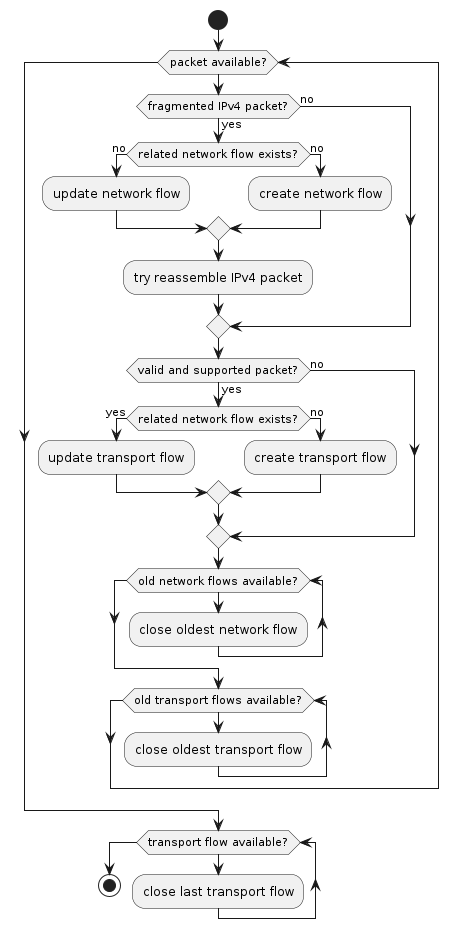
\includegraphics{plant_uml_diagrams/general_tool_loop.png}
    }
  \end{center}
  \caption{Flujo de la aplicación durante su ejecución}\label{fig:packet_pincer_execution}
\end{figure}


\subsection{Argumentos de consola y señales}

Por hacer

\subsection{Lectura de paquetes en tiempo real}

Por hacer

\subsection{Lectura de trazas de paquetes}

Por hacer

\subsection{Extensión de libreria de código abierto para la decodificación de paquetes}

Por hacer

\subsection{Defragmentación IPv4}

Por hacer

\subsection{Separación de flujos}

Por hacer

\subsection{Generación de estadísticas}

Por hacer

\subsection{Escritura y etiquetado de flujos}

Por hacer

